\chapter{مروری بر کارهای پیشین}
\label{chap:relatedworks}
مسئله‌ی بهینه‌سازی شبکه‌های تلفن همراه از جنبه‌های مختلفی موردمطالعه قرار گرفته است که می‌توان آن‌ها را در دسته‌بندی‌های گوناگونی قرار داد. از دیدگاه جمع‌آوری داده به جهت بهینه‌سازی، می‌توان آن را به دو دسته‌ی جمع‌آوری داده سمت 
\gls{UE} 
و جمع‌آوری داده سمت شبکه دسته‌بندی کرد. عملیات  \gls{DriveTest} از جمله روش‌های جمع‌آوری داده سمت \gls{UE} و \gls{MDT} از جمله روش‌های جمع‌آوری داده سمت شبکه است. در 
\autoref{fig:relatedWorksRoadmap}
حوزه‌های مختلف بهینه‌سازی که در ادامه‌ی این فصل مورد بررسی قرار می‌گیرند، قابل‌مشاهده است. 

\begin{figure}
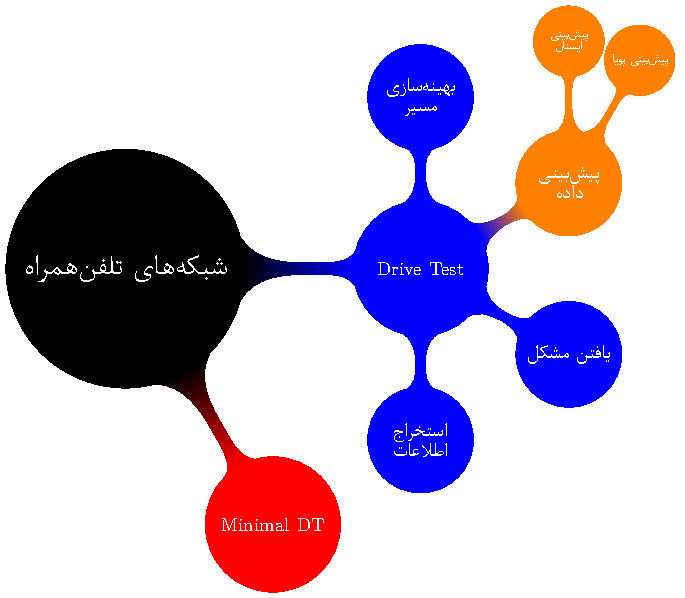
\includegraphics[width=0.65\linewidth]{/Roadmap/mainFig}
\caption{\lofimage{/Roadmap/mainFig}%
حوزه‌های بهینه‌سازی شبکه‌های تلفن همراه از دیدگاه جمع‌آوری داده}
\label{fig:relatedWorksRoadmap}
\end{figure}


\section{بهینه‌سازی مسیر}
\begin{figure}
\begin{subfigure}[b]{.24\textwidth}\centering
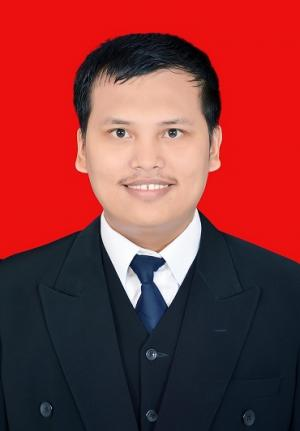
\includegraphics[height = .9\linewidth]{/Person/LukmanMedriavinSilalahi}
\caption{\lr{L. Medriavin Silalahi \cite{silalahi2021improvement}}}
\end{subfigure} 
\begin{subfigure}[b]{.24\linewidth}\centering
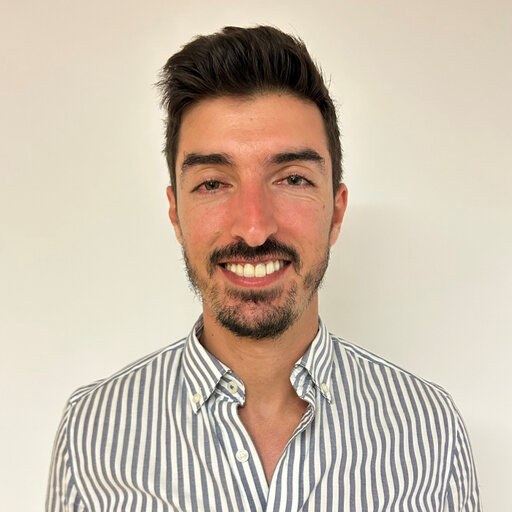
\includegraphics[height=0.9\linewidth]{/Person/MarcoSousa}
\caption{\lr{Marco Sousa \cite{Sousa2021Analysis}}}
\end{subfigure}
\begin{subfigure}[b]{.24\linewidth}\centering
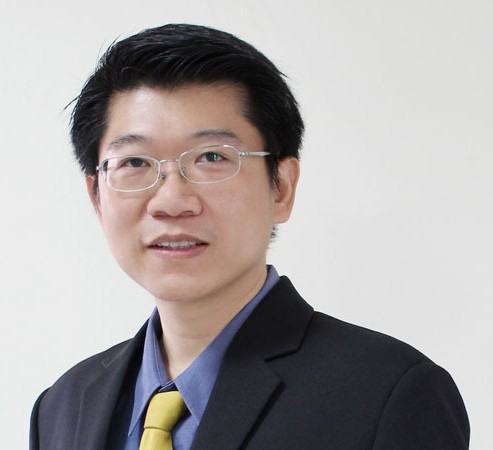
\includegraphics[height=0.9\linewidth]{/Person/peeraponguthansakul}
\caption{\lr{Peerapong Uthansakul \cite{charoenlap2016prediction}}}
\end{subfigure}
\begin{subfigure}[b]{.24\linewidth}\centering
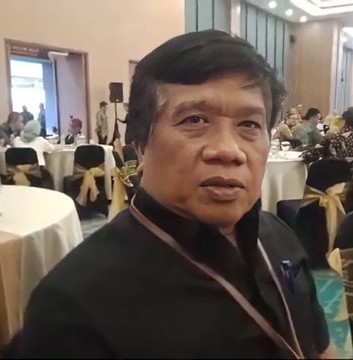
\includegraphics[height=0.9\linewidth]{/Person/YuliarmanSaragih}
\caption{\lr{Yuliarman Saragih \cite{Aprillia2020RF}}}
\end{subfigure}
\end{figure}


\section{حل مشکلات}